\appendix
\chapter{Appendix}
\section{Mesh properties}
The presented meshes still have to be overlaid with the level set which defines the calculation region. The level set that was used has been specified in the specification of the corresponding simulations.
	\begin{figure}[htp]
		\centering
		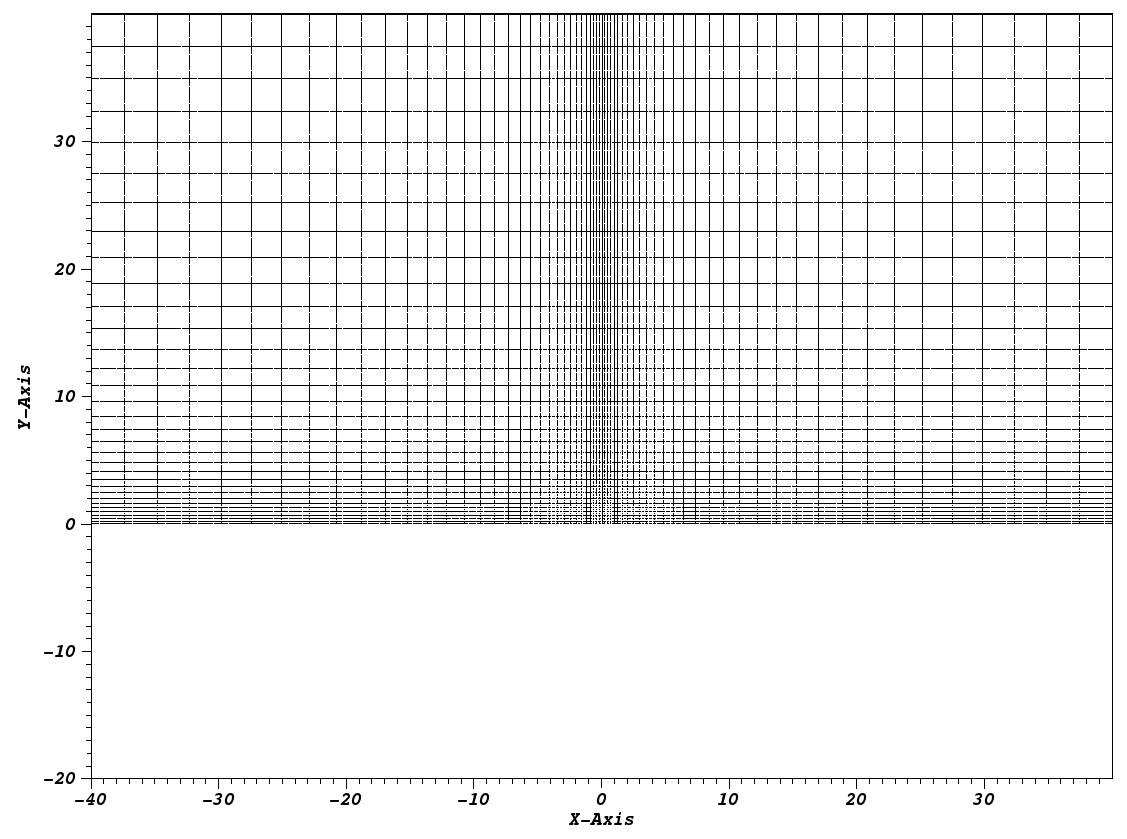
\includegraphics[height=7cm]{eulershift.PNG}
		\caption{Mesh Used in the Robustness Study}
		\label{fig:eulershift}
	\end{figure}  
	\begin{figure}[htp]
		\centering
		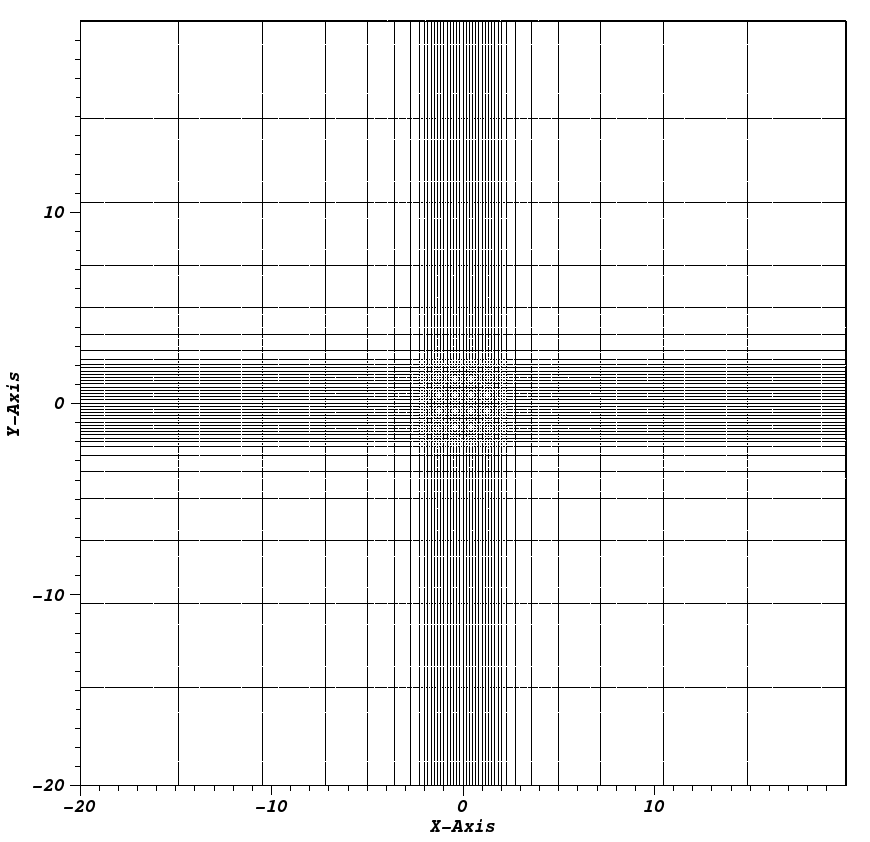
\includegraphics[height=7cm]{CpD40.PNG}
		\caption{Mesh for CpD40}
		\label{fig:ms40}
	\end{figure}
	\begin{figure}[htp]
		\centering
		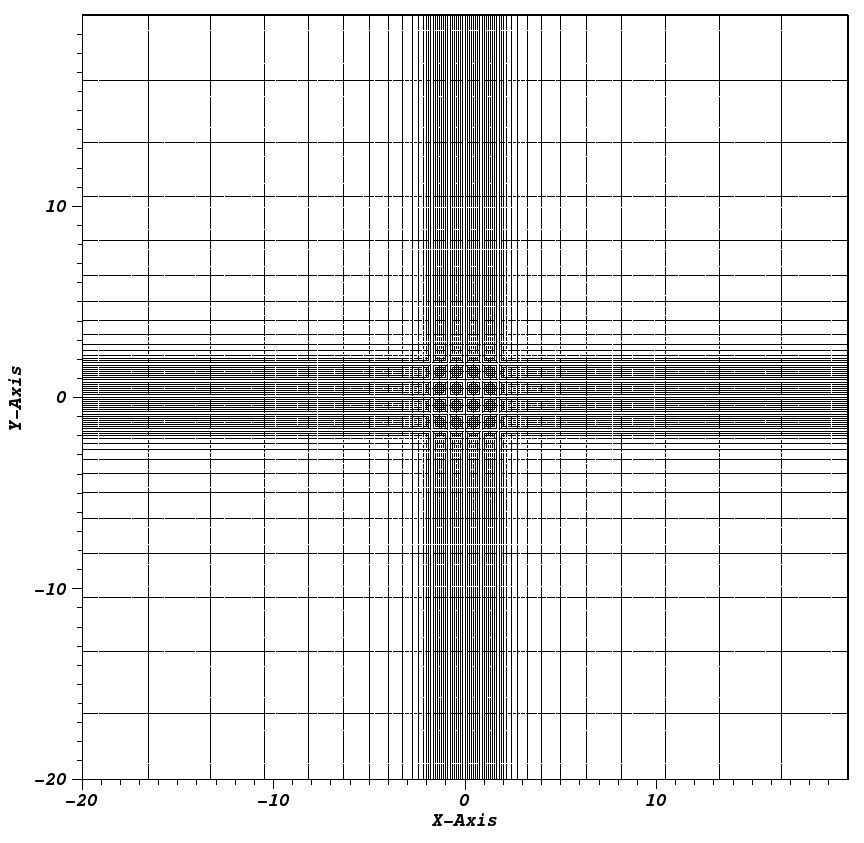
\includegraphics[height=7cm]{CpD60.PNG}
		\caption{Mesh for CpD60}
		\label{fig:ms60}
	\end{figure} 
	\begin{figure}[htp]
		\centering
		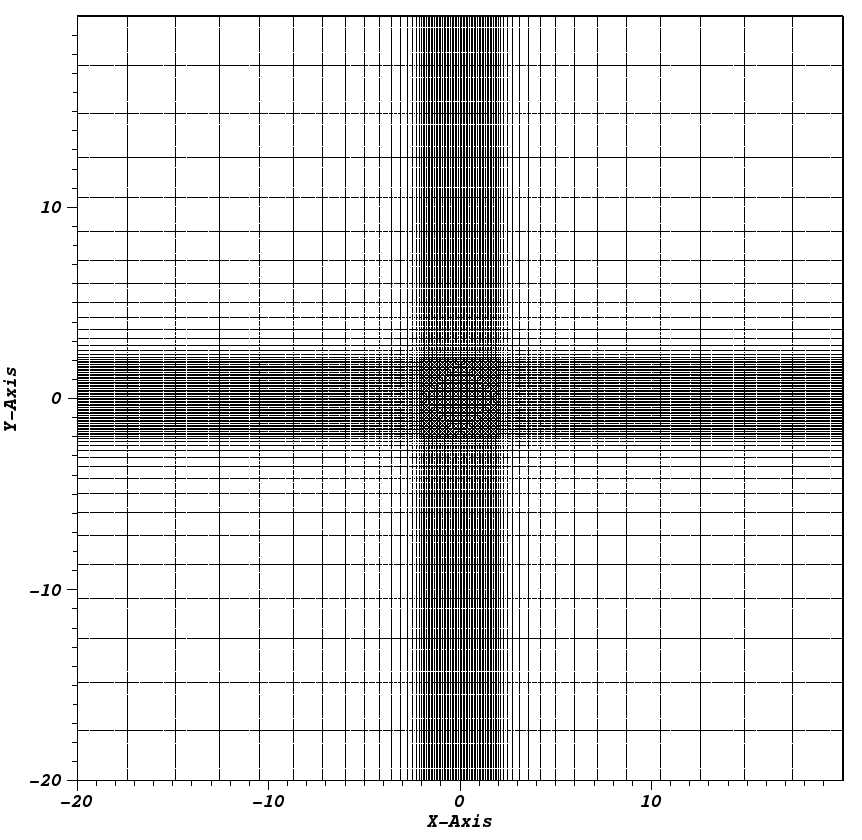
\includegraphics[height=7cm]{CpD80.PNG}
		\caption{Mesh for CpD80}
		\label{fig:ms80}
	\end{figure}  